\documentclass[a4paper,12pt]{report}
\addtolength{\oddsidemargin}{-1.cm}
\addtolength{\textwidth}{2cm}
\addtolength{\topmargin}{-2cm}
\addtolength{\textheight}{3.5cm}
\newcommand{\HRule}{\rule{\linewidth}{0.5mm}}
\makeindex

\usepackage{longtable}
\usepackage[pdftex]{graphicx}
\usepackage{makeidx}
\usepackage{hyperref}
\usepackage{float}
\hypersetup{
    colorlinks=true,
    linkcolor=black,
    filecolor=magenta,      
    urlcolor=cyan,
}

\setcounter{secnumdepth}{3}

\DeclareGraphicsExtensions{.pdf,.png,.jpg}
% define the title
\author{Neo Tandem Technologies}
\title{ Functional Specification - Eye Tracking}
\begin{document}
\setlength{\parskip}{6pt}

% generates the title
\begin{titlepage}

\begin{center}
% Upper part of the page       

\includegraphics[scale=1]{../GeneralImages/up-logo.jpg}
\\[1cm]    
    

\textsc{\LARGE Neo Tandem Technologies}\\[1.5cm]
%\textsc{\Large Eye Tracking}\\[0.5cm]
%\textsc{\Large Architectural Specification}\\[0.5cm]

\includegraphics[scale=0.2]{../GeneralImages/NTT.jpg}\\[1.5cm]
% Title
\HRule \\[0.4cm]
{ \huge \bfseries Eye Tracking}\\[0.4cm]
\HRule \\[0.4cm]
% Author and supervisor
\begin{minipage}{0.4\textwidth}
\begin{flushleft} \large
\emph{Author:}\\
Duran {Cole}
\end{flushleft}
\end{minipage}
\begin{minipage}{0.4\textwidth}
\begin{flushright} \large
\emph{Student number:} \\
u13329414
\end{flushright}
\end{minipage}
\begin{minipage}{0.4\textwidth}
\begin{flushleft} \large
Michael {Nunes}
\end{flushleft}
\end{minipage}
\begin{minipage}{0.4\textwidth}
\begin{flushright} \large
\emph{} \\
u12104592
\end{flushright}
\end{minipage}
\begin{minipage}{0.4\textwidth}
\begin{flushleft} \large
Molefe {Molefe}
\end{flushleft}
\end{minipage}
\begin{minipage}{0.4\textwidth}
\begin{flushright} \large
\emph{} \\
u12260429
\end{flushright}
\end{minipage}
\begin{minipage}{0.4\textwidth}
\begin{flushleft} \large
Tebogo {Seshibe}
\end{flushleft}
\end{minipage}
\begin{minipage}{0.4\textwidth}
\begin{flushright} \large
\emph{} \\
u13181442
\end{flushright}
\end{minipage}
\begin{minipage}{0.4\textwidth}
\begin{flushleft} \large
Timothy {Snayers}
\end{flushleft}
\end{minipage}
\begin{minipage}{0.4\textwidth}
\begin{flushright} \large
\emph{} \\
u13397134
\end{flushright}
\end{minipage}
\vfill
% Bottom of the page
{\large \today}
\end{center}
\end{titlepage}
\footnotesize
%\input{declaration_of_originality.tex}
\normalsize

\renewcommand{\thesection}{\arabic{section}}
\newpage
\begin{center}
\textsc{\LARGE Architecture requirements}\\[1.5cm]
\textsc{\Large Eye Tracking}\\[0.5cm]

Github Link:

Version: Version 0.2 Alpha 
\today
\end{center}
\tableofcontents{}


\section{Architecture requirements}

\subsection{Quality Requirements}
	%\documentclass{a4paper,12pt}{report}
%\addtolength{\textwidth}{2cm}
%\addtolength{\topmargin}{-2cm}
%\addtolength{\textheight}{3.5cm}
%\newcommand{\HRule}{\rule{\linewidth}{0.5mm}}

%\begin{document}

\subsubsection{Scalability}
\begin{flushleft}
The requirements for scalability in the program are that the storage of all the data will forever expand with the more uses of the program. This means that the longer you have the system the more data it will take up, this then states that we need to ensure that later on the space will not impact on the users performance. The program itself can also grow in terms of features. This means that a developer can extend system by adding a new feature.
\begin{itemize}
\item{Tactics and strategies}
\begin{itemize}
\item{Compression}: Compression of the files will allow more files to be stored on a hard drive. This can lead to greater scalability and improve space management.
\end{itemize}

\item{Integration}: The integration of scalability in our system will allow the users to decide where the files that are written will be saved. This will enable them to save the files to hard-drives as time with the system goes on. This allows the user to expand their storage capacity. \\
The system is also created in a way that everything is a module/component. The program allows for new modules to be created and then added. This encourages the growth of the system from the start as new and better components can be added.
\end{itemize}

\end{flushleft}
		
\subsubsection{Performance}
\begin{flushleft}
Performance of the system is key as the system is constantly reading in data as the eye is being tracked so the performance needs to be optimized so that the tracking of the eye does not stutter and then incorrectly track the eye. The system also needs to perform well and not cause issues when it is run.
\begin{itemize}
\item{Tactics and strategies}:
\begin{itemize}
\item{Thread pooling}: this will allow us to spread the work load across threads so that they can run concurrently and reduce bottlenecks. This also allows us to optimize how we can use the hardware so that we use it to its maximum potential. The Eye Tribe SDK handles threading that is related to eye tracking by creating separate threads for gaze listeners.
\end{itemize}

\item{Integration}: The system will be able to run the server that will get gaze data to run concurrently with the eye tracking function.Each of these is run on a thread and this allows them to run at the same time so all the data is collected in real time and the performance is optimized.\\
The system is spread into components which means that each component is responsible for a task and this increases performance as there are not waiting processes.
\end{itemize}

\end{flushleft}
		
\subsubsection{Maintainability}
\begin{flushleft}
The system will need to be maintained over time as new technologies are introduced.The system is component based which makes maintainability easier as the components need to be maintained and not the entire system.Maintainability allows a program to be kept up-to-date. Changes in eye tracking is a common thing so we expect new changes to occur frequently.
\begin{itemize}
\item{Tactics and strategies}
\begin{itemize}
\item{Removal of Faulty Components}: This allows us to remove components that are no longer working in the system and then replace them with a newer version of them all and if needs be a whole new type of component.
\item{Deadlock Detection}: The detection of deadlock is important and if a deadlock occurs could harm your system.This is important as detecting a deadlock can also then determine if the component is faulty.
\end{itemize}

\item{Integration}: The system is component based so removing and maintaining the system is made easier.If we know that a certain part of the system is causing a problem such as deadlock or is faulty in any other way we can then  decide to remove that component and fix it or add a new system. This way changes are made to a component and not the whole system.
\end{itemize}

\end{flushleft}
		
\subsubsection{Reliability and Availability}	
\begin{flushleft}
Reliability and Availability are important in this system. The server which is used for capturing the data needs to constantly be available to the program so that data can be read.The program also needs to be reliable and gather the information correctly. The collection of incorrect data can cause mishaps with the system. The system as a whole needs to be running and not crash and fail.
\begin{itemize}
\item{Tactics and strategies}
\begin{itemize}
\item{Load Balancing}: By balancing the work load we can ensure that a system can continuously run and not have a crash. This call also cause services to constantly be available such as the server.
\item{Removal of Faulty Components}: The removing of faulty components allows us to increase the reliability of the system by removing the cause of the unreliability.
\end{itemize}

\item{Integration} :
The load balancing can be achieved by separating the specific tasks into different components.This allows the system to share the load across different sub sections. The removal of the components can be done manually so that the system does not contain the faulty component.
\end{itemize}

\end{flushleft}	
		
\subsubsection{Security}	
\begin{flushleft}
The system is connected to the server and this can lead to a security threat as the connection can be compromised and allow an attack on a user. This is a security concern as the system can be indirectly used to harm the user of the system.
\begin{itemize}
\item{Tactics and strategies}
\begin{itemize}
\item{Request/Connection Dropping}: Dropping the connection to the server can then reduce the risk of a users security to be compromised and thus increasing security. The system must also be secure as not to harm the hardware itself and to also not damage any accompanying hardware such as the eye tracker. The tracker can also be used by a malicious user to spy on the systems users.

\end{itemize}

\item{Integration}: When the system no longer needs to use the the server to get the data the system must cut the connection to the server and then restart the connection once the server will start connecting once more to the server. This reduces the risk of the channel being used by someone malicious and harming the users of the system.
\end{itemize}

\end{flushleft}	

\subsubsection{Usability}
\begin{flushleft}
When a user needs the system it will need to be usable, in other words the program should allow the user to explore all the features of the system and be able to use them all.
\begin{itemize}
\item{Tactics and strategies}
\begin{itemize}
\item{Contracts based decoupling}: The system is decoupled by dividing the system into a set of contracts that each have its specification and have its pre- and post-conditions. This allows the system to be easily decoupled.

\end{itemize}

\item{Integration}: The contracts created are used to make the system in to components which allows new contracts to be created as the system develops and there is no tight coupling amongst all the components hence there is no reliance on them.
\end{itemize}

\end{flushleft}
		
\subsubsection{Testability and Integrability}
\begin{flushleft}
The system is quite a large system and the testing would need to be done on every aspect of the system this would mean that the system would need to have testing done all over. The system also needs to be integrated with all the systems components and this would mean that the system would need a high level of integration.
\begin{itemize}
\item{Tactics and strategies}
\begin{itemize}
\item{Layering}: This will allow each component to be comprised of a layer and this layer can then be changed or removed. This allows good integration in the components.

\end{itemize}

\item{Integration}: Each layer will have a set of components and these components can be changed and then integrated easily with the layers that are next to them. This allows the system to ave easy integration and allows changes to the system not effect the integration.The testing is made easy with each component allowed to be tested on individually so that the integration can be done seamlessly.
\end{itemize}

\end{flushleft}
		
\subsection{Integration and access channel requirements}
	\subsubsection{Access channel requirements}

\subsubsection{Channels}

\subsubsection{Protocols}

\subsubsection{API Specifications}

\subsection{Architecture constraints}
	\subsubsection{Hardware}
The Eye Tribe eye tracking device will be used as the primary eye tracking recording device for this project. The Eye Tribe eye tracking device connects to the computer through a USB 3.0 port and as such it is required that the computer the application would be running on has USB 3.0 ports.

\subsubsection{Operating System}
The application only supports installation on computers running a Microsoft Windows operating system. The application may work on both 32-bit and 64-bit systems but 64-bit systems with large amounts of memory are recommended for memory processing. 

\subsubsection{Additional Software}
You need to have the .Net 4.0 Framework installed or better to run the program. This ensures that all the current technologies are used properly and to the best of their ability. The Eye tribe SDK will also need to be installed so that the camera can be calibrated and data can be transferred to the program.

\subsubsection{Version Control Management}
GitHub will be used to as the version control management system for the duration of this project.
This is a distributed version control meaning that every node has a copy of the repository. With this tool we can easily track issues and bug fixes throughout the program as well as manage new features and testing with the use of branches.

\subsubsection{Development Environment}
The application will be programmed in the C sharp(C\#) programming language through Microsoft Visual Studio 2013 Community Edition. This is a free version of Microsoft's Visual studio and is built for small development teams such as up to five members. The additional software (namely The Eye Tribe SDK) being used also provides C\# libraries that can be used to access additional features and capabilities of their software and hardware.

\section{Architectural patterns or styles}
	\subsection{Singleton Recorder}
The program uses a server to gather and record the data from the eye tracking camera. This server is constantly running and there should only be one instance of this class running so that we do not have multiple servers running and all the data is pulled consistently from one location. The server will thus need to follow the singleton design pattern. The singleton design pattern is a creational design pattern that is used when only one instance of the object should be created for the application. This will provide the solution of only one server object being created at time. It will check whether an instance of the requested object is created and if it is the object is referenced and not recreated and therefore there can only be one instance of the class created.

	\begin{figure}[!ht]
		\centering
		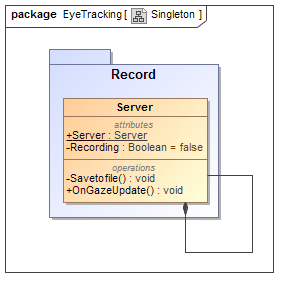
\includegraphics[scale=0.5]{Diagrams/Class_Diagram__Singleton.png}
		\caption{Singleton Recorder}
	\end{figure}


%\subsection{Extensibility pattern}
%The program is comprised of many different modules to increase the re-usability of the different developed code. The different modules will need to work together to perform all the tasks that the program is required to carry out. The extensibility pattern helps to achieve this. The extensibility pattern provides a framework for the inclusion of other modules into the program. This is achieved through C\# and its ability to create DLL (Dynamic Link library) for use in another solution. This allows us to very easily add functionality and will also allow the fixing and enhancing of the application at a later stage without affecting any other working modules. Meaning that modules can be easily added and removed from the system with little negative affect.
%

\subsection{Flyweight Settings}
The program has data that needs to be shared amongst modules and that also needs to be used through-out the system. This is achieved by use of the flyweight pattern. The application requires all system and model settings to be created, saved and eventually used by the rest of the modules within the system. These variables are static and are defined as internal so that only the program can access the stored setting values. This ensures that all the modules are able to read and change the shared memory resource.

\begin{figure}[!ht]
		\centering
		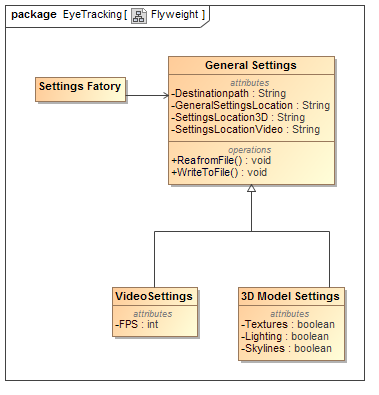
\includegraphics[scale=0.5]{Diagrams/Class_Diagram__Flyweight.png}
		\caption{Flyweight Settings}
	\end{figure}


%\subsection{Model-View-Controller} 
%\begin{flushleft}
%The project can easily be split as: User, Interface and, Background Calculations. The user interacts %with the Interface, the program that will be executed, handling the eye tracking. The interface will %convert the received data into a format that the data processing section can work with. The data %processing section will take render out/back the heat maps generate from the users focus.

%It is with this in mind that the Model-View-Controller(MVC) design pattern will be used.
%The MVC separates the data model, user interface, and control logic which is exactly what we want. We %want the user to be able to use our system without having to know how it works. Only the basics %should be available i.e record, printing out texture/model.
%\end{flushleft}

\subsection{Composite}
With in our program we have built a graphics module with the help of OpenTK that allows us to render three-dimensional (3D) models, preform actions on them and return desired results. When it comes to building the model we first have to import it and start the process of parsing the model into data we can use to create a visual representation. Each model is saved in an object file (".obj") this file contains a parent game-object and its multiple children game-objects. This pattern creates a tree of each game-objects and its sub-game-objects.

\begin{figure}[!ht]
	\centering
	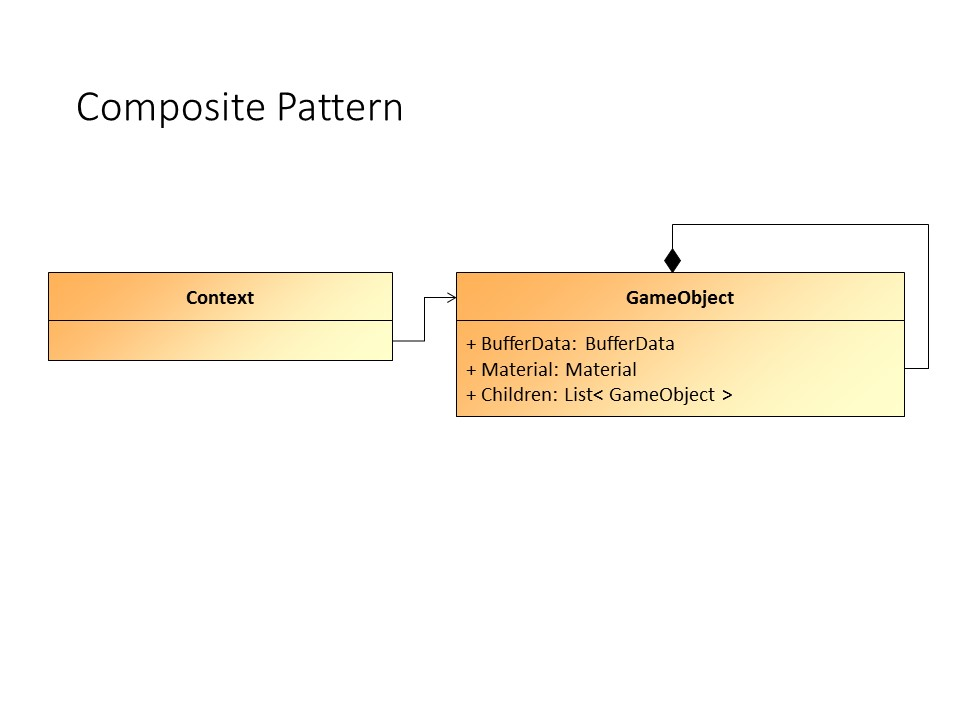
\includegraphics[scale=0.5]{Diagrams/Slide4.jpg}
	\caption{Composite Game-Objects}
\end{figure}


\subsection{Private Class}
This pattern gives the system a means of separating all game-objects and their attributes into different containers and thus aids in simplifying the class definition.

\begin{figure}[!ht]
	\centering
	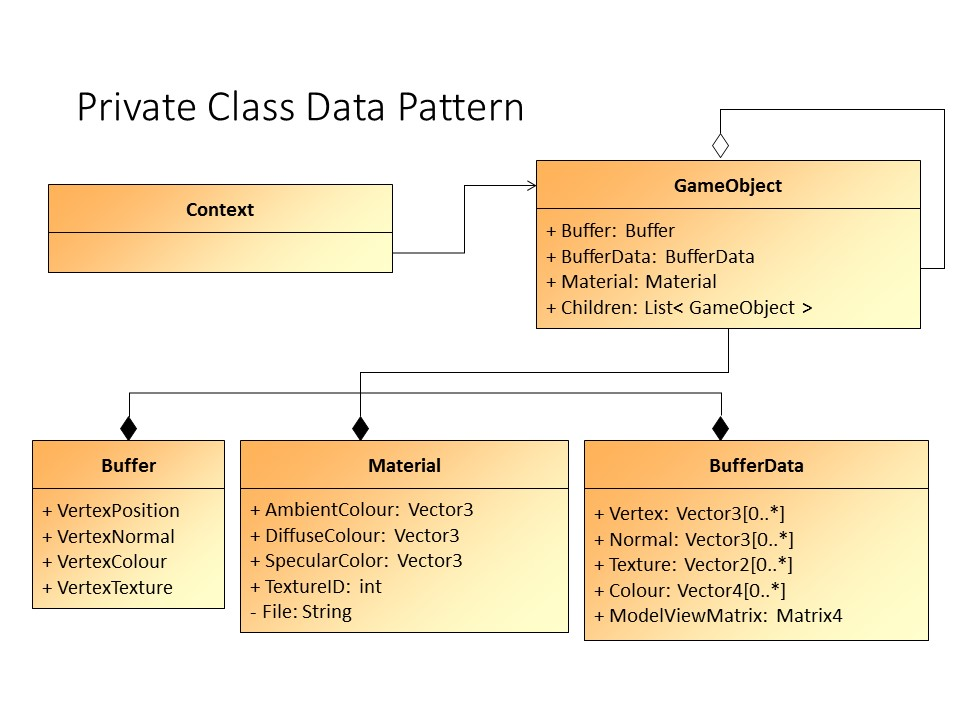
\includegraphics[scale=0.5]{Diagrams/Slide5.jpg}
	\caption{Private Class Game-Objects}
\end{figure}

\subsection{Facade}
When you wish to import and view a model the first action that will occur is a call to the display model class. The facade will call a converter to parse the object file and call the game window to render the object. This pattern hides the complexity of both generation and rendering the model by just providing a single, simple entry point.

\begin{figure}[!ht]
	\centering
	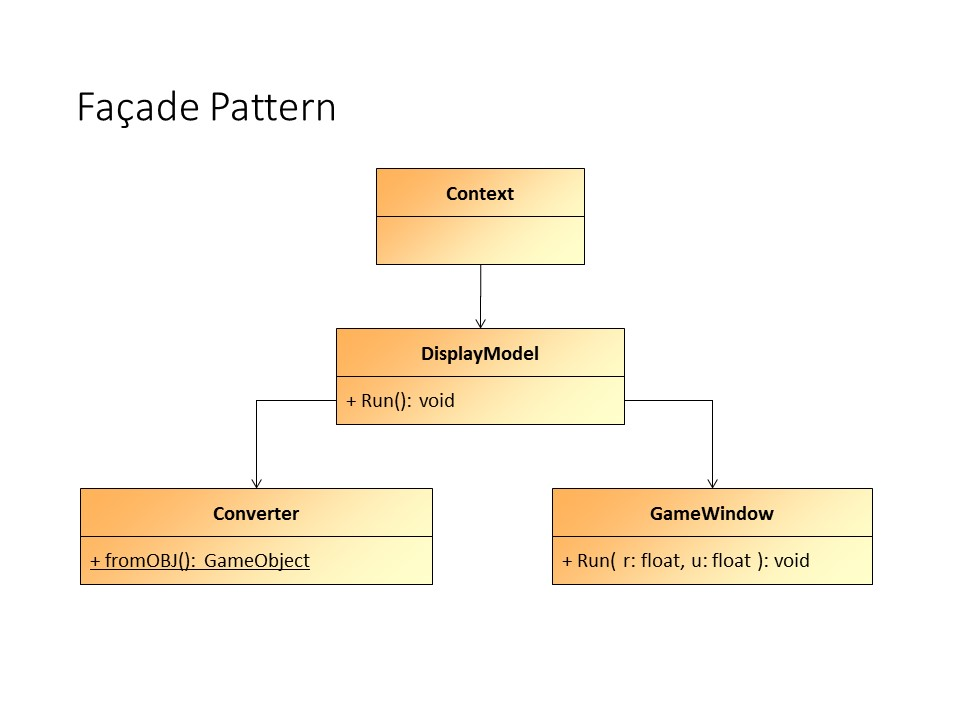
\includegraphics[scale=0.5]{Diagrams/Slide6.jpg}
	\caption{Facade Game-Objects}
\end{figure}

\subsection{Template Method}
With in the space of three-dimensional models multiple features can be applied, such as different lighting techniques. The pattern consists of the base light class which is an abstraction of its three sub-classes. In the system we make use of this pattern to decide what type of lighting will be applied to a model. There are three types of lighting, namely: ambient, point and directional lighting. A combination of any three can be used but currently all three are being utilised.

\begin{figure}[!ht]
	\centering
	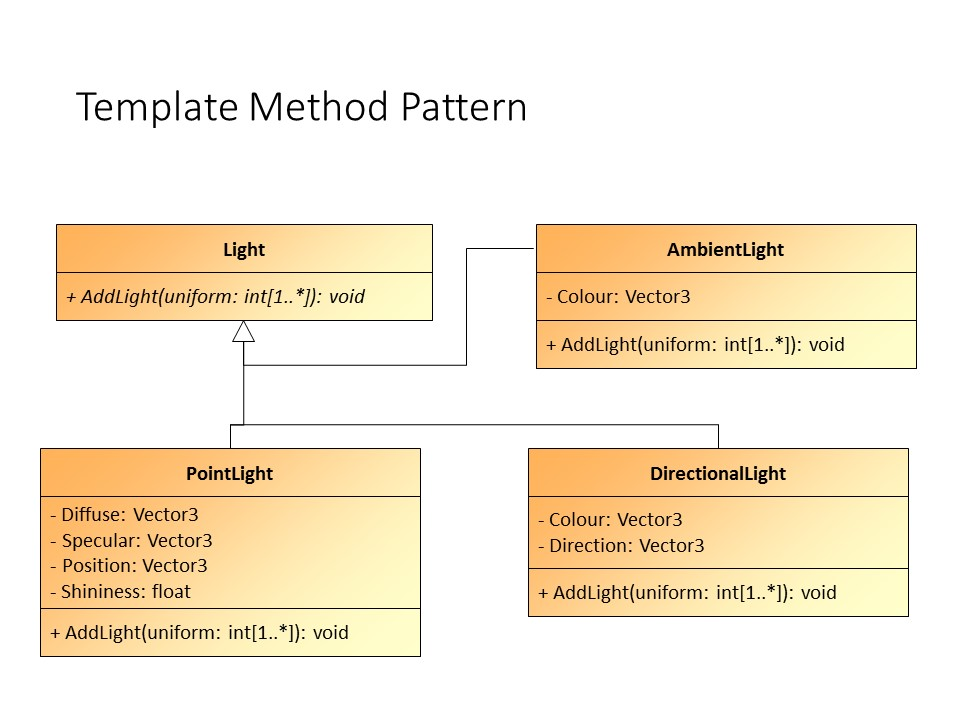
\includegraphics[scale=0.5]{Diagrams/Slide8.jpg}
	\caption{Template Method Game-Objects}
\end{figure}

\subsection{Builder}
As multiple different three dimensional objects models can be imported all with different structures and objects, we make use of the builder design pattern to separate the construction of each game-objects so that each object can be built dynamically based on its requirements. A three dimensional object consists of a buffer, vertex buffer objects, materials and a list of children objects. When parsing the parsing the ".obj" file all objects are created, followed by the parsing of the ".mtl" file where all materials are created and attached to the objects. The root object and its tree structure is then generated and returned.

\begin{figure}[!ht]
	\centering
	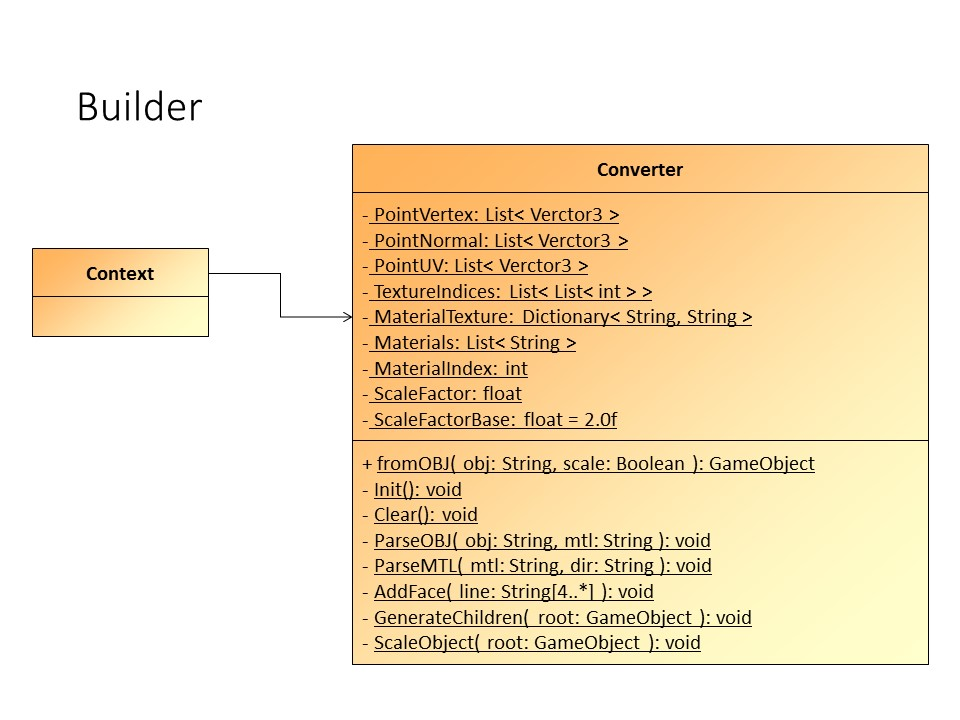
\includegraphics[scale=0.5]{Diagrams/Slide9.jpg}
	\caption{Builder Game-Objects}
\end{figure}
\section{Architectural tactics or strategies}
	\subsection{Availability}
This refers to whether the user will have constant access to the program and methods to avoid interruptions.

Because of the way in which the system will work, all aspects of the systems will be working as long as it is running. Therefore, an exception based fault detection system is required to ensure nothing fails. Unless it is the user interface that fails, the exception will be handle the error in the background, and a connection between the sections of the systems will be re-attempted.

Checkpoints will be saved in order to roll back in the event of errors.

\subsection{Scalability}
This refers to time and cost relating to development, changes, and testing of the system.

The MVC pattern allows us to separate concerns of the system allowing for finer grain implementation and changes to its inner working. This will also allow for potential changes to be "plugged in" if required.

This is also means that testing will be easy as each section simply needs to test whether they are able to do their own required task. All related task will simply be using the abstraction of the subsystem.

\subsection{Performance}
This refers to the speed of execution, the time between a request and a response between modules within the system.

In order to simplify the subsystems, any optimized, pre-existing algorithms that can help with their executions will be used. The least possible intermediaries will be used. Concurrency will also be used in sections to ensure speed of generation when it comes to creating heat maps and gaze plot.
\iffalse
\subsection{Security}
This refers to the safety of the data that the system will be used.

The system is to be designed in such a way that no users can interfere with the inner workings of the subsystems. The overall purpose of this systems is to provide extra functionality to a device and so, changes to how it works are not required.
\fi
\subsection{Testability}
This refers to the ease of testing of the system, during successive build releases.

During each build release, all test cases used in the subsystems unit tests, will be combined into a series of big test cases in order to make sure that the expected input provides the same expected output.

\subsection{Usability}
This refers to the ease of use the user will have with regards to the system.

Since the system will be doing most of the work, the user will only be provided with a very simple interface to interact with the basic functions i.e. record screen, print to texture.

\section{Use of reference architectures and frameworks}
	\subsubsection{Reference Architecture}
\begin{flushleft}
Say what you want to say for the reference architecture

\end{flushleft}
\section{Technologies}
	We have chose the following technologies carefully as they incorporate into one another to form a sound basis for our project to operate on.

\begin{itemize}
	\item \textbf{C\#}:	C\# is a programming language that was designed and developed by Microsoft.The language is a object orientated language and is highly focused on component-oriented. C\# is used with the .NET frame work which was discussed in a earlier section. The language is a very versatile language that is used when developing most Microsoft projects. The language is able to create classes and a GUI which allows us to map certain functions of the GUI to the class.
	
	\item \textbf{Eye Tribe eye-tracker}: This is one of the cheapest if not the cheapest eye tracking cameras available on the market.The tracker is infra-red eye tracker which can track gaze data and then this data can be used to carry out numerous functions.The Eye tribe eye tracker can be used on a computer or a mobile device such as a smart phone.The eye tracker is \$99 eye tracker that makes it cheap and competitive with the more expensive ones on the market.
	
	\item \textbf{Eye tribe SDK}: This is a full SDK that is used to develop programs that will use the Eye-tribe tracking camera. The SDK comes with the user interface and server components to help design new programs that are compatible with the eye tribe software.
	
	\item \textbf{GitHub}: This is a version control system that is used to manage the versions of software.Github uses a copy-modify-merge system where the users will clone a repository and then modify it and then merge it. It is a distributed version control so every person has copy to the repository.
		\item \textbf{NuGet}: This is a packet manager which helps to manage all the packages in a project. This allows users to add packages from all sources to their projects to use certain parts of it.This also manages the packages so that you don't have to worry about locating them and referencing them.
		\item \textbf{Nunit}: This is a testing framework built for the .Net framework.This is very similar to java's JUnit. The same premise and method is used to create and execute tests. The tests will show a positive result if they have passed.If a failure occurs on a test it will tell you where and what cause the error. NUnit is used to write unit tests so that each part of a project is tested.
		
		\item \textbf{OpenTK}: OpenTK or Open Toolkit Library is a OpenGL library that allows the users to manipulate 3D models inside a .Net projects such as a C\# project. This means that a 3D model can then be manipulated and used in a program.
		
		\item \textbf{Visual Studio Community 2013}: Visual Studio Community 2013 is a robust IDE used to write .NET projects such as a C\#  project.The IDE has many features that help improve development and increase productivity. The Visual Studio community edition is free to developers if you sign up with a Microsoft account.
\end{itemize}
% Workin with references
% here we add our citations	
\begin{thebibliography}{9}

  	
\end{thebibliography}
\end{document}
